%%%%%%%%%%%%%%%%%%%%%%%%%%%%%%%%%%%%%%%%%%%%%%%%%%%%%%
% A Beamer template for University of Wollongong     %
% Based on THU beamer theme                          %
% Author: Qiuyu Lu                                   %
% Date: July 2024                                    %
% LPPL Licensed.                                     %
%%%%%%%%%%%%%%%%%%%%%%%%%%%%%%%%%%%%%%%%%%%%%%%%%%%%%%
% Customized for Sharif University of Technology     %
%%%%%%%%%%%%%%%%%%%%%%%%%%%%%%%%%%%%%%%%%%%%%%%%%%%%%%


\documentclass[serif, aspectratio=169]{beamer}
%\documentclass[serif]{beamer}  % for 4:3 ratio
\usepackage[T1]{fontenc} 
\usepackage{fourier} % see "http://faq.ktug.org/wiki/uploads/MathFonts.pdf" for other options
\usepackage{hyperref}
\usepackage{latexsym,amsmath,xcolor,multicol,booktabs,calligra}
\usepackage{graphicx,pstricks,listings,stackengine}
\usepackage{lipsum}
\usepackage{tikz}
\usetikzlibrary{arrows.meta, positioning}

\author{Ali Sharifi-Zarchi}
\title{Machine Learning (CE 40717)}
\subtitle{Fall 2024}
\institute{
    CE Department \\
    Sharif University of Technology
}
%\date{\small \today}
% \usepackage{UoWstyle}
\usepackage{SUTstyle}

% defs
\def\cmd#1{\texttt{\color{red}\footnotesize $\backslash$#1}}
\def\env#1{\texttt{\color{blue}\footnotesize #1}}
\definecolor{deepblue}{rgb}{0,0,0.5}
\definecolor{deepred}{RGB}{153,0,0}
\definecolor{deepgreen}{rgb}{0,0.5,0}
\definecolor{halfgray}{gray}{0.55}

\lstset{
    basicstyle=\ttfamily\small,
    keywordstyle=\bfseries\color{deepblue},
    emphstyle=\ttfamily\color{deepred},    % Custom highlighting style
    stringstyle=\color{deepgreen},
    numbers=left,
    numberstyle=\small\color{halfgray},
    rulesepcolor=\color{red!20!green!20!blue!20},
    frame=shadowbox,
}


\begin{document}



\begin{frame}
    \titlepage
    \vspace*{-0.6cm}
    \begin{figure}[htpb]
        \begin{center}
            
\includegraphics[keepaspectratio, scale=0.25]{pic/sharif-main-logo.png}
        \end{center}
    \end{figure}
\end{frame}

\begin{frame}
    \centering
    These slides were prepared with contributions from Aren Golazizian
\end{frame}

\begin{frame}    
\tableofcontents[sectionstyle=show,
subsectionstyle=show/shaded/hide,
subsubsectionstyle=show/shaded/hide]
\end{frame}

\section{Transformers}

\begin{frame}{Attention is All You Need!}
    \begin{figure}
        \centering
        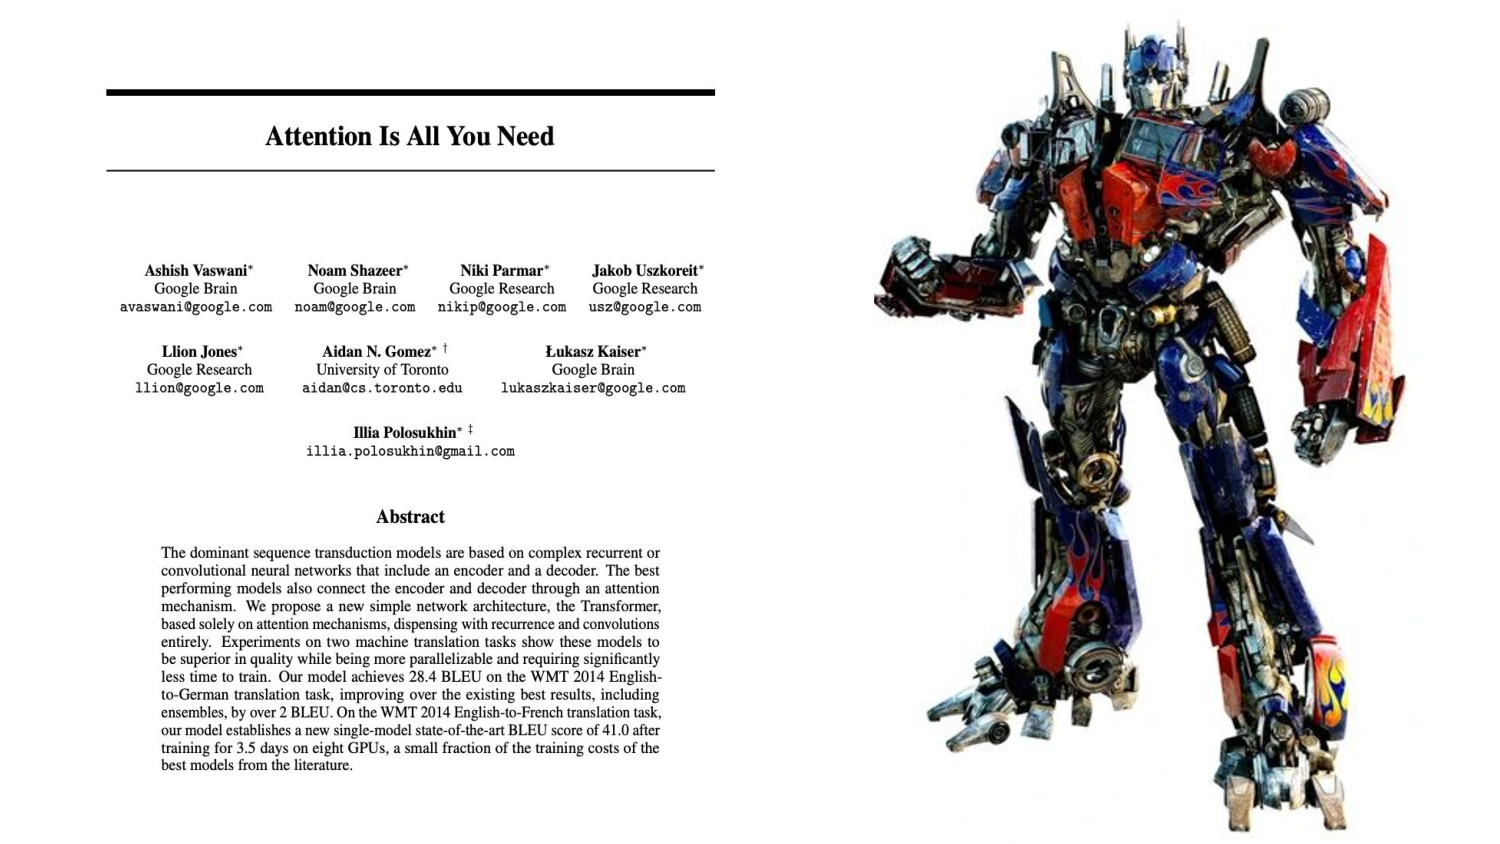
\includegraphics[width=0.9\linewidth]{Figures/Untitled presentation (2).pdf}
        \label{fig:enter-label}
    \end{figure}
    \begin{tikzpicture}[remember picture,overlay]
        \node[anchor=south west, xshift=0.09cm, yshift=0.3cm] at (current page.south west) {\tiny \href{https://arxiv.org/abs/1706.03762}{https://arxiv.org/abs/1706.03762}};
    \end{tikzpicture}
\end{frame}
\newpage

\begin{frame}{Transformer Architectures}
    \begin{figure}
        \centering
        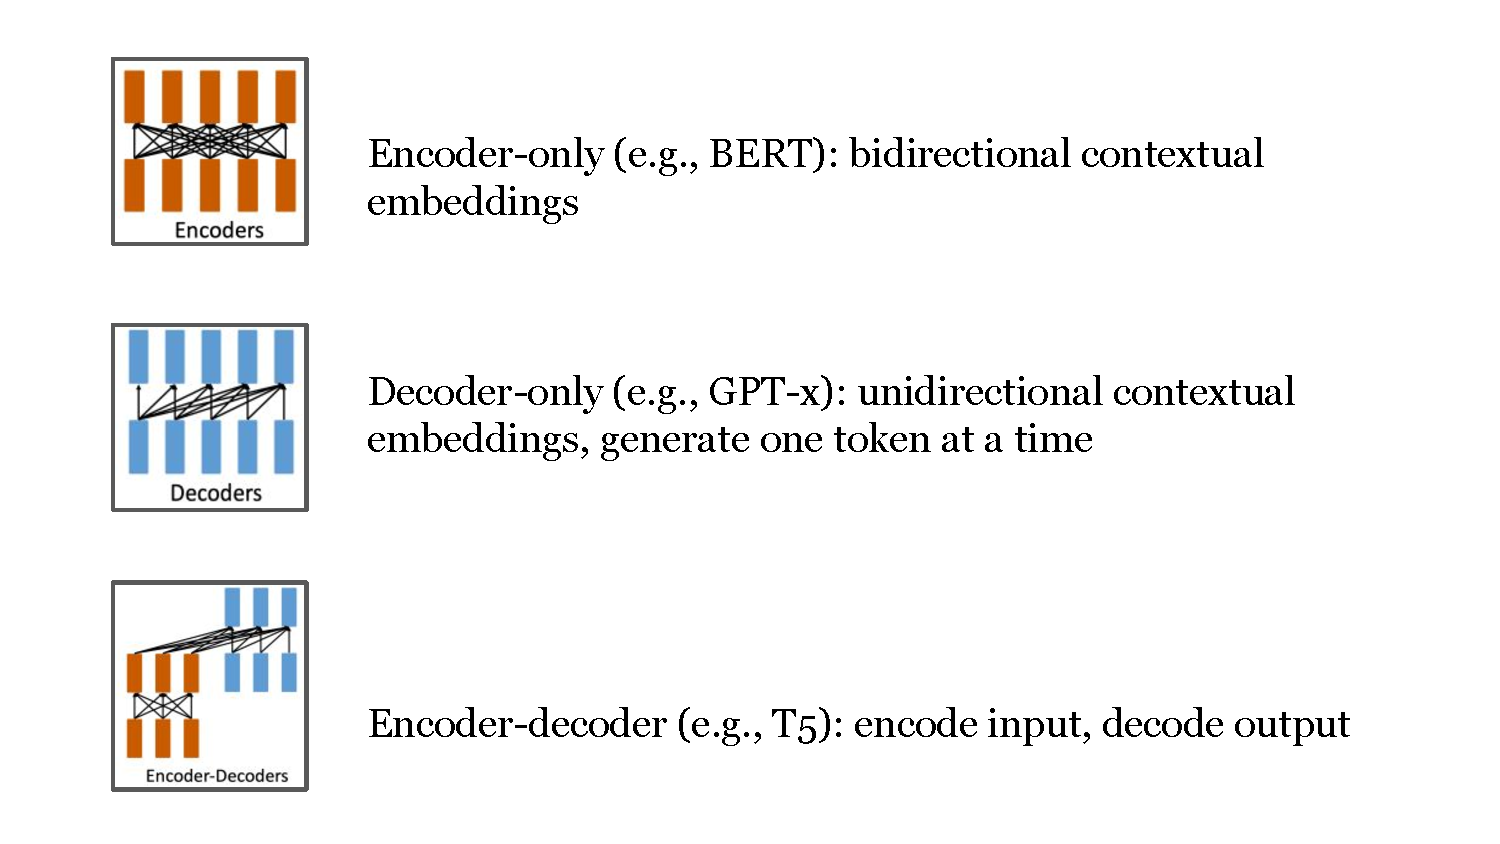
\includegraphics[width=0.9\linewidth]{Figures/Untitled presentation (3).pdf}
        \caption{Enter Caption}
        \label{fig:enter-label}
    \end{figure}
\end{frame}

\begin{frame}{Transformer block}
    \begin{columns}
        \column{.55\textwidth}
        \begin{itemize}
            \item Each block has two "sublayers"
            \begin{itemize}
                \item[]  1.Multihead attention
                \item[] 2.Feed-forward Neural Network (with ReLU)
            \end{itemize}
            \item Residual: x + Sublayer(x)
            \item Layer Normalization changes input to have mean 0 and variance 1
        \end{itemize}
        \column{.45\textwidth}
        \centering
        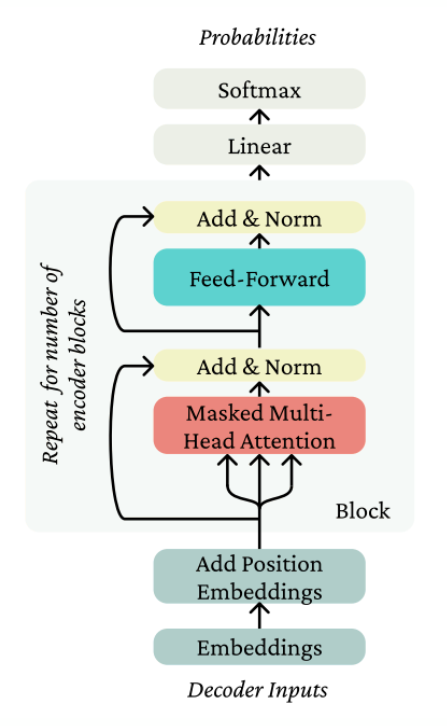
\includegraphics[width=.6\linewidth]{Figures/transformer-block.png}
    \end{columns}
    \begin{tikzpicture}[remember picture,overlay]
        \node[anchor=south west, xshift=0.3cm, yshift=0.3cm] at (current page.south west) {\tiny \href{https://web.stanford.edu/class/cs224n/slides/cs224n-2024-lecture19-open-problems.pdf2}{https://web.stanford.edu/class/cs224n/slides/cs224n-2024-lecture19-open-problems.pdf}};
    \end{tikzpicture}
\end{frame}

\begin{frame}{Layer normalization}
    \textbf{Main Idea:} Batch normalization is advantageous for stability but presents challenges with sequences of varying lengths. \\
    \textbf{Result:} It provides a more stable input for the next layer. \\
    \textbf{Solution:} "Layer normalization" functions similarly to batch normalization but doesn't normalize across the entire batch.
    
    \vspace{0.5cm}
    
    \begin{columns}
        % Batch Norm Column
        \column{.6\textwidth}
        \centering
        \textbf{\Large Batch norm}
        
        \begin{align*}
            \mu &= \frac{1}{B} \sum_{i=1}^{B} a_i, \quad \sigma = \sqrt{\frac{1}{B} \sum_{i=1}^{B} (a_i - \mu)^2} \\
            \bar{a}_i &= \frac{a_i - \mu}{\sigma}
        \end{align*}
        
        \textit{d-dimensional vectors for each sample in batch}

        % Layer Norm Column
        \column{.5\textwidth}
        \centering
        \textbf{\Large Layer norm}
        
        \begin{align*}
            \mu &= \frac{1}{d} \sum_{i=1}^{d} a_j, \quad \sigma = \sqrt{\frac{1}{d} \sum_{i=1}^{d} (a_j - \mu)^2} \\
            \bar{a} &= \frac{a - \mu}{\sigma}
        \end{align*}
        
        \textit{Different dimensions of a}
    \end{columns}
    
\end{frame}

\begin{frame}{Why Transformers?}
    \Huge
    \textbf{Why Transformers?}
    
    \vspace{0.5cm}
    
    \large
    \textbf{Pros:}
    \begin{itemize}
        \item[] {\color[rgb]{0,0.5,0}+ Much easier to parallelize}
        \item[] {\color[rgb]{0,0.5,0}+ Much better long-range connections}
        \item[] {\color[rgb]{0,0.5,0}+ In practice, can make it much deeper (more layers) than RNN}
    \end{itemize}
    
    \vspace{0.5cm}
    
    \textbf{Cons:}
    \begin{itemize}
        \item[] {\color{red}- Attention computations are technically$O(n^2)$}
        \item[] {\color{red}- Somewhat more complex to implement (positional encodings, etc.)}
    \end{itemize}
\end{frame}

\section{Encoder Architecture}

\begin{frame}{Encoder Language Model}
    \begin{figure}
        \centering
        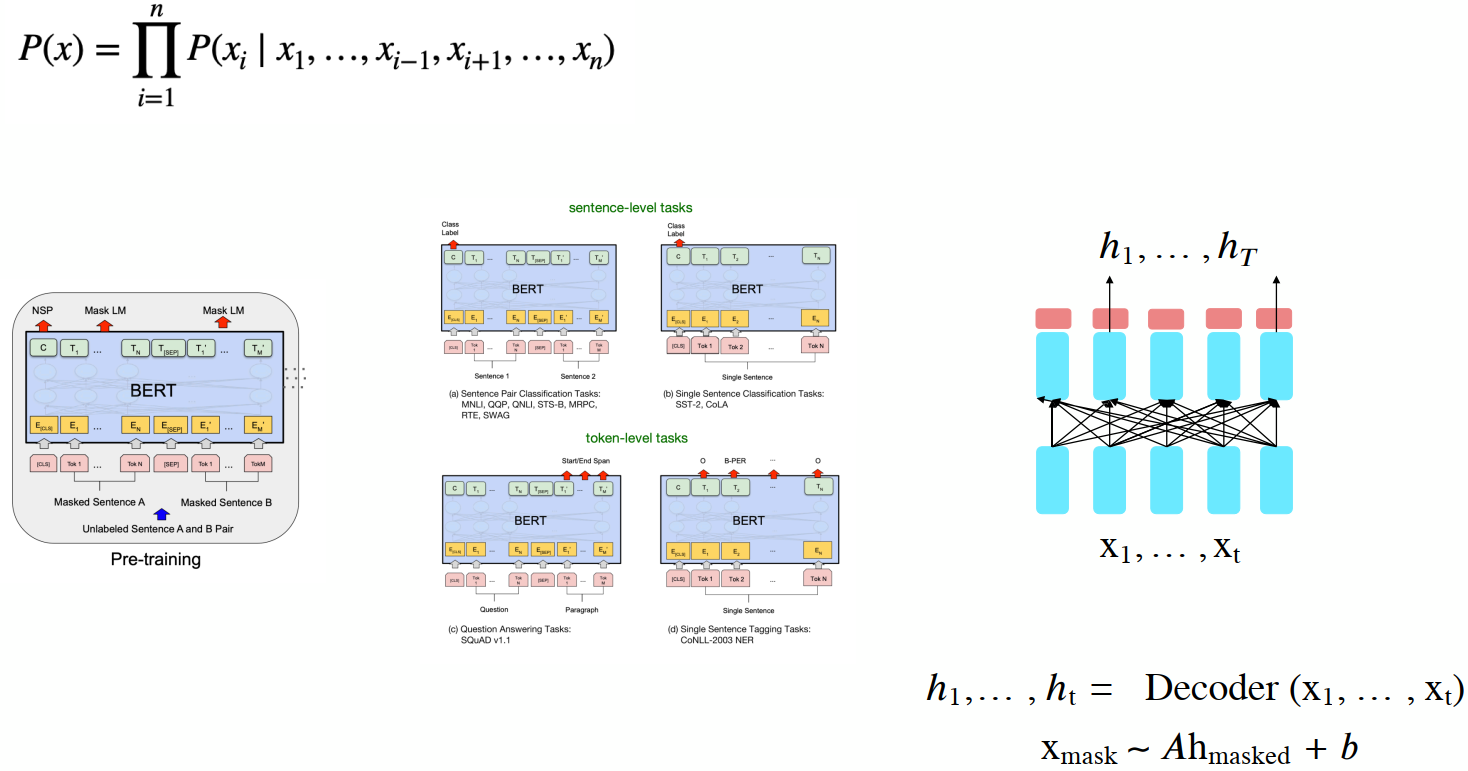
\includegraphics[width=0.9\textwidth]{Figures/encoderlm.png}
    \end{figure}
    \begin{tikzpicture}[remember picture,overlay]
        \node[anchor=south west, xshift=0.09cm, yshift=0.3cm] at (current page.south west) {\tiny \href{   https://arxiv.org/abs/1810.04805}{   https://arxiv.org/abs/1810.04805}};
    \end{tikzpicture}
\end{frame}

\begin{frame}{Encoder Language Model}
    % Short Description
    Encoder language models, like BERT, use masked tokens to learn bidirectional representations of text.
    % Bullet Points for Additional Explanation
    \vspace{0.5cm}
    \begin{itemize}
        \item \textbf{Masked Language Modeling (MLM):} Predicts randomly masked tokens in a sequence.
        \item \textbf{Bidirectional Context:} Considers information from both directions for each token.
        \item \textbf{Applications:} Used for classification, NER, and other NLP tasks.
    \end{itemize}
\end{frame}

\begin{frame}{BERT: Key Contributions}
    
    \vspace{0.5cm}
    
    \begin{itemize}
        \item It is a fine-tuning approach based on a deep Transformer Encoder.
        
        \vspace{0.3cm}
        
        \item The key: learn representations based on \textbf{bidirectional context}
        
        \vspace{0.2cm}
        
        \textcolor{green!50!black}{
        Why? Because both left and right contexts are important to understand the meaning of words.}
        
        \vspace{0.2cm}
        
        Example \#1: we went to the river \textcolor{red}{bank}. \\
        Example \#2: I need to go to \textcolor{red}{bank} to make a deposit.
        
        \vspace{0.5cm}
        
        \item \textbf{Pre-training objectives:} masked language modeling + next sentence prediction
        
        \vspace{0.3cm}
        
        \item State-of-the-art performance on a large set of \textbf{sentence-level} and \textbf{token-level} tasks
    \end{itemize}
    
\end{frame}

\begin{frame}{BERT pre-training: putting together}
    \begin{columns}
        % Left Column - Image
        \column{.4\textwidth}
        \begin{figure}[h]
            \centering
            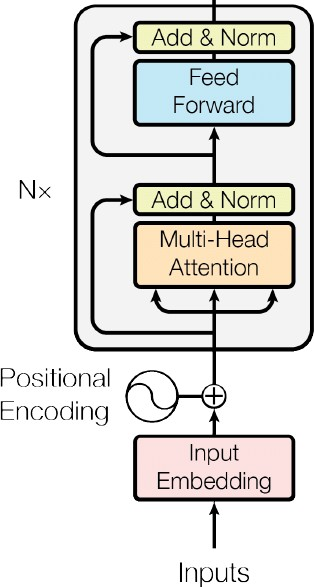
\includegraphics[width=0.5\textwidth]{Figures/BERT.png}
        \end{figure}
        
        % Right Column - Bullet Points
        \column{.6\textwidth}
        \begin{itemize}
            \item \textbf{BERT-Base:} 12 layers, 768 hidden size, 12 attention heads, 110M parameters
            \vspace{0.3cm}
            \item \textbf{BERT-Large:} 24 layers, 1024 hidden size, 16 attention heads, 340M parameters
            \vspace{0.3cm}
            \item \textbf{Training corpus:} Wikipedia (2.5B) + BooksCorpus (0.8B)
            \vspace{0.3cm}
            \item \textbf{Max sequence size:} 512 word pieces (roughly 256 and 256 for two non-contiguous sequences)
            \vspace{0.3cm}
            \item \textbf{Trained for:} 1M steps, batch size 128k
        \end{itemize}
    \end{columns}
    \begin{tikzpicture}[remember picture,overlay]
        \node[anchor=south west, xshift=0.09cm, yshift=0.3cm] at (current page.south west) {\tiny \href{   https://arxiv.org/abs/1706.03762}{   https://arxiv.org/abs/1706.03762}};
    \end{tikzpicture}
\end{frame}

\begin{frame}{Sentence-level tasks}
    \begin{figure}
        \centering
        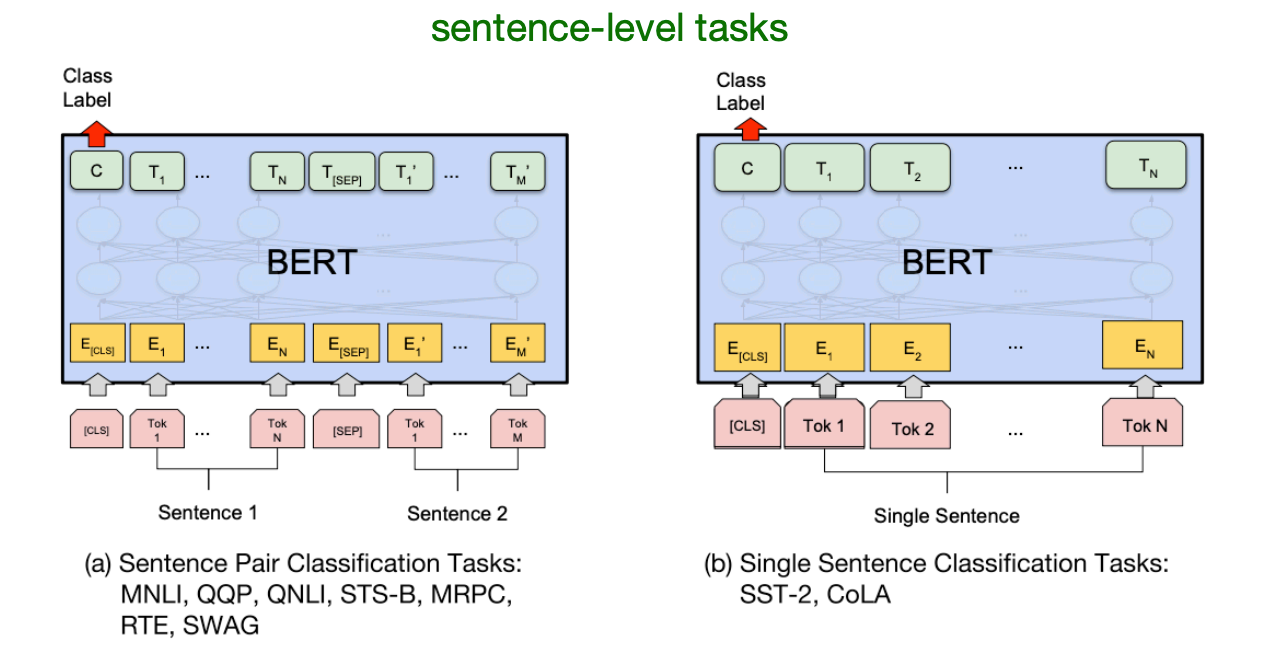
\includegraphics[width=0.9\textwidth]{Figures/sentence-level-tasks.png}
    \end{figure}
    \begin{tikzpicture}[remember picture,overlay]
        \node[anchor=south west, xshift=0.09cm, yshift=0.3cm] at (current page.south west) {\tiny \href{   https://arxiv.org/abs/1810.04805}{   https://arxiv.org/abs/1810.04805}};
    \end{tikzpicture}
\end{frame}

\begin{frame}{Sentence-level tasks(cont.)}
    \begin{itemize}
        % Sentence pair classification tasks
        \item Sentence pair classification tasks:
        \begin{itemize}
            % MNLI example
            \item[] \setlength{\fboxsep}{2pt}\colorbox{yellow!30}{\textbf{MNLI}}
            \begin{itemize}
                \item \textbf{Premise:} A soccer game with multiple males playing.
                \item \textbf{Hypothesis:} Some men are playing a sport.
                \item Result: \{\textcolor{green!50!black}{\underline{\text{entailment}}}, contradiction, neutral\}
            \end{itemize}

            \item[] \setlength{\fboxsep}{2pt}\colorbox{yellow!30}{\textbf{QQP}}
            \begin{itemize}
                \item Q1: Where can I learn to invest in stocks?
                \item Q2: How can I learn more about stocks?
                \item Result: \{\textcolor{green!50!black}{\underline{\text{duplicate}}}, not duplicate\}

            \end{itemize}
        \end{itemize}
        
        % Single sentence classification tasks
        \item Single sentence classification tasks:
        
        \begin{itemize}
            % SST2 example
            \item[] \setlength{\fboxsep}{2pt}\colorbox{yellow!30}{\textbf{SST2}}
            \begin{itemize}
                \item Sentence: rich veins of funny stuff in this movie
                \item Result: \{\textcolor{green!50!black}{\underline{\textcolor{green!50!black}{positive}}}, negative\}

            \end{itemize}
        \end{itemize}
    \end{itemize}
    
\end{frame}

\begin{frame}{Token-level tasks}
    \begin{figure}
        \centering
        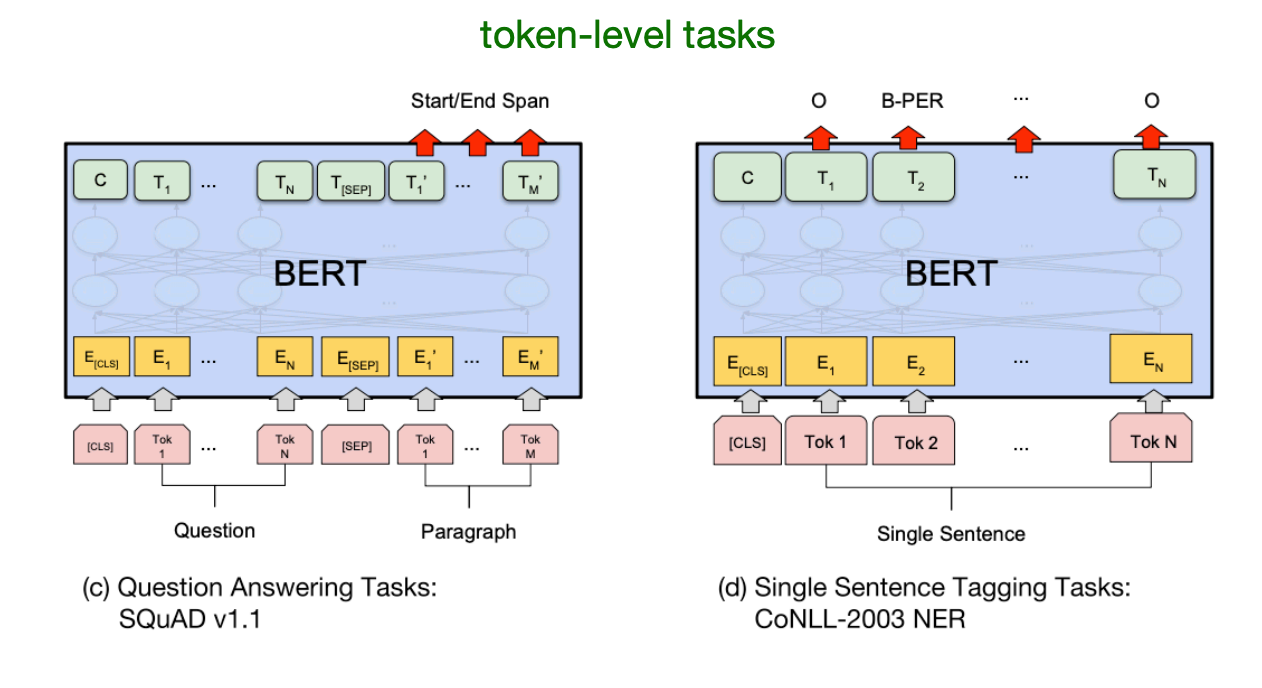
\includegraphics[width=0.9\textwidth]{Figures/token-level-tasks.png}
    \end{figure}
    \begin{tikzpicture}[remember picture,overlay]
        \node[anchor=south west, xshift=0.3cm, yshift=0.3cm] at (current page.south west) {\tiny \href{   https://arxiv.org/abs/1810.04805}{   https://arxiv.org/abs/1810.04805}};
    \end{tikzpicture}
\end{frame}

\begin{frame}{Token-level tasks: Extractive Question Answering}

    % Extractive Question Answering
    \begin{itemize}
        \item Extractive question answering e.g., SQuAD (\textcolor{green!50!black}{Rajpurkar et al., 2016})
    \end{itemize}
    
    % SQuAD Example
    \begin{itemize}
        \item[] \setlength{\fboxsep}{2pt}\colorbox{yellow!30}{\textbf{SQuAD}}
    \end{itemize}
    
    \vspace{0.2cm}
    
    \begin{figure}[h]
        \centering
        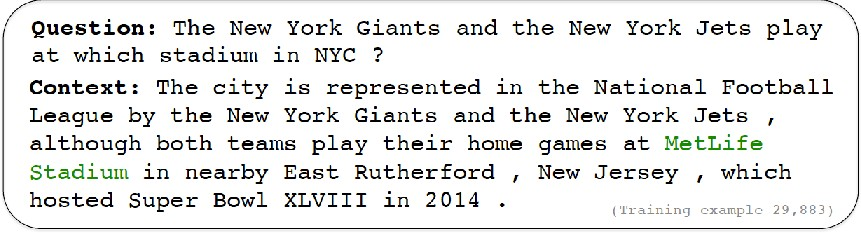
\includegraphics[width=0.9\textwidth]{Figures/tk-task.png}
    \end{figure}
    
    \hspace{1cm} Example Result: MetLife Stadium
\end{frame}

\begin{frame}{Token-level tasks: Named Entity Recognition}
    \textbf{Token-level tasks}
    
    \vspace{0.5cm}
    
    % Named Entity Recognition
    \begin{itemize}
        \item Named entity recognition (\textcolor{green!50!black}{Tjong Kim Sang and De Meulder, 2003})
    \end{itemize}
    
    \vspace{0.3cm}
    
    % CoNLL 2003 Example
    \begin{itemize}
        \item[] \setlength{\fboxsep}{2pt}\colorbox{yellow!30}{\textbf{CoNLL 2003 NER}}
    \end{itemize}
    
    \vspace{0.3cm}
    
    \begin{center}
        \begin{tabular}{c c c c c c}
            John & Smith & lives & in & New & York \\
            B-PER & I-PER & O & O & B-LOC & I-LOC
        \end{tabular}
    \end{center}
    
\end{frame}

\begin{frame}{Masked Language Modeling (MLM)}
    \begin{itemize}
        \item \textbf{Q:} Why we can’t do language modeling with bidirectional models?
    \end{itemize}
    
    \begin{figure}[h]
        \centering
        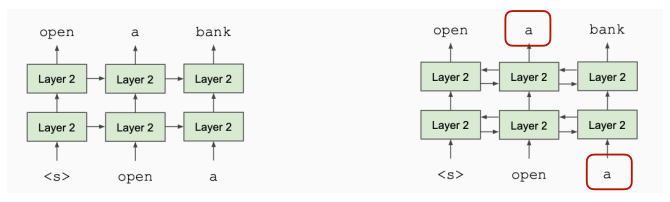
\includegraphics[width=0.8\textwidth]{Figures/MLM.png}
    \end{figure}
    
    \begin{itemize}
        \item \textbf{Solution:} Mask out a percentage k of the input words, and then predict the masked words.
    \end{itemize}
    
    \vspace{0.3cm}
    
    \begin{center}
        \begin{tabular}{c c c c}
            & \textbf{store} && \textbf{gallon} \\
            & $\downarrow$ && $\downarrow$ \\
            the man went to & $[MASK]$ & to buy a & $[MASK]$ of milk
        \end{tabular}
    \end{center}
\end{frame}

\begin{frame}{MLM: Masking Rate and Strategy}
    \begin{itemize}
        \item \textbf{Q: What is the value of k?}
        \begin{itemize}
            \item They always use $k = 15\%$.
            \item Too little masking: computationally expensive (we need to increase \# of epochs)
            \item Too much masking: not enough context
            \item See \textcolor{green!50!black}{(Wettig et al., 2022)} for more discussion of masking rates:
            \begin{itemize}
                \item Masking 40\% outperforms 15\% for BERT-large size models on GLUE and SQuAD
                \item High masking rate of 80\% can still preserve 95\% fine-tuning performance
            \end{itemize}
        \end{itemize}
        
        \vspace{0.5cm}
        
        \item \textbf{Q: How are masked tokens selected?}
        \begin{itemize}
            \item 15\% tokens are uniformly sampled
            \item Is it optimal? See span masking \textcolor{green!50!black}{(Joshi et al., 2020)} and PMI masking \textcolor{green!50!black}{(Levine et al., 2021)}
        \end{itemize}
    \end{itemize}
    
    \vspace{0.5cm}
    
    \textbf{Example:} He \textbf{[MASK]} from Kuala \textbf{[MASK]}, Malaysia.
    
\end{frame}

\begin{frame}{Next Sentence Prediction (NSP)}
    \begin{itemize}
        \item Motivation: many NLP downstream tasks require understanding the relationship between two sentences (natural language inference, paraphrase detection, QA).
        \item NSP is designed to reduce the gap between pre-training and fine-tuning.
    \end{itemize}
    \begin{figure}
            \centering
            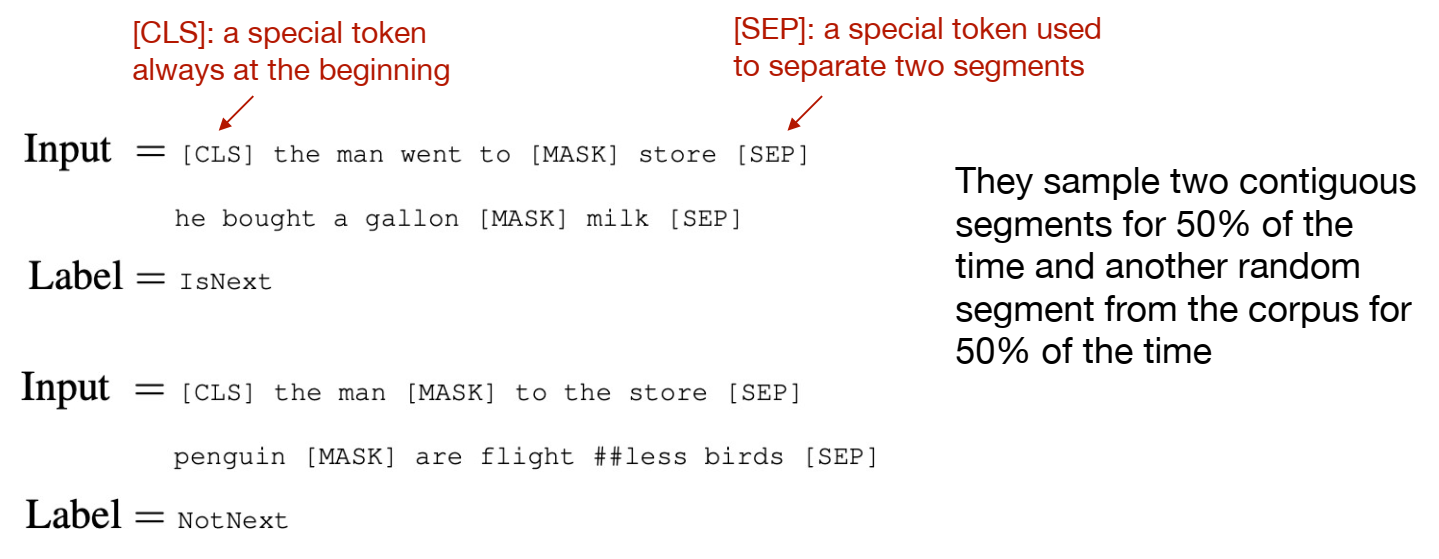
\includegraphics[width=0.9\textwidth]{Figures/NSP.png}
    \end{figure}
\end{frame}

\begin{frame}{BERT Training}

    \vspace{0.5cm}
    
    \textbf{Dataset:} Let $\mathcal{D}$ be a set of examples $(x_{1:L}, c)$ constructed as follows:
    
    \vspace{0.3cm}
    
    \begin{itemize}
        \item Let $A$ be a sentence from the corpus.
        \item With probability 0.5, let $B$ be the next sentence.
        \item With probability 0.5, let $B$ be a random sentence from the corpus.
        \item Let $x_{1:L} = [\text{CLS}], A, [\text{SEP}], B$.
        \item Let $c$ denote whether $B$ is the next sentence or not.
    \end{itemize}
    
    \textbf{Objective.} Then the BERT objective is:
    \begin{figure}
            \centering
            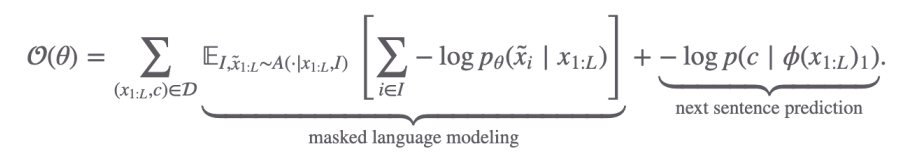
\includegraphics[width=0.9\textwidth]{Figures/Objective.png}
    \end{figure}

\end{frame}

\begin{frame}{BERT Pre-training: Putting Together}
    \begin{itemize}
        \item \textbf{Vocabulary size:} 30,000 wordpieces (common sub-word units) \textcolor{green!50!black}{(Wu et al., 2016)}
    \end{itemize}
    
    \begin{figure}
        \centering
        % Placeholder for the first image
        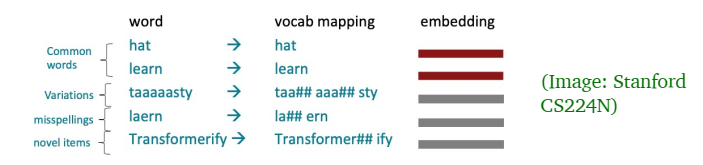
\includegraphics[width=0.7\textwidth]{Figures/input embeddings.png}
    \end{figure}
    
    \begin{itemize}
        \item \textbf{Input embeddings:}
    \end{itemize}
    
    \begin{figure}
        \centering
        % Placeholder for the second image
        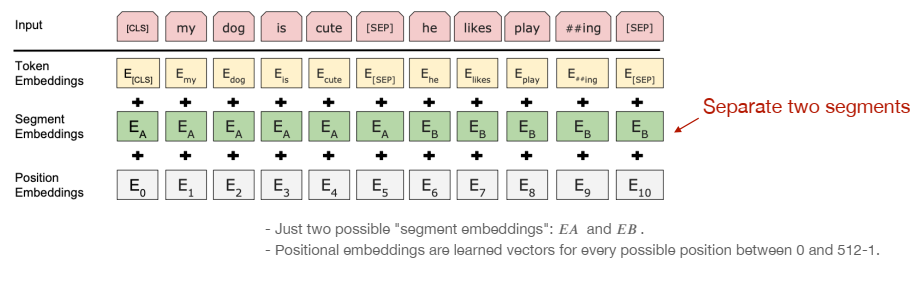
\includegraphics[width=0.8\textwidth]{Figures/voc.png}
    \end{figure}
    \begin{tikzpicture}[remember picture,overlay]
        \node[anchor=south west, xshift=0.08cm, yshift=0.3cm] at (current page.south west) {\tiny \href{https://cs330.stanford.edu/fall2019/presentations/presentation-10.23-1.pdf}{https://cs330.stanford.edu/fall2019/presentations/presentation-10.23-1.pdf}};
    \end{tikzpicture}
\end{frame}

\begin{frame}{BERT Pre-training: Putting Together}
    \begin{columns}
        % Left column with text
        \begin{column}{0.5\textwidth} % Specify the width for the first column
            \begin{itemize}
                \item MLM and NSP are trained together
                \item \texttt{[CLS]} is pre-trained for NSP
                \item Other token representations are trained for MLM
            \end{itemize}
        \end{column}
        
        % Right column with image
        \begin{column}{0.5\textwidth}
            \begin{figure}
                \centering
                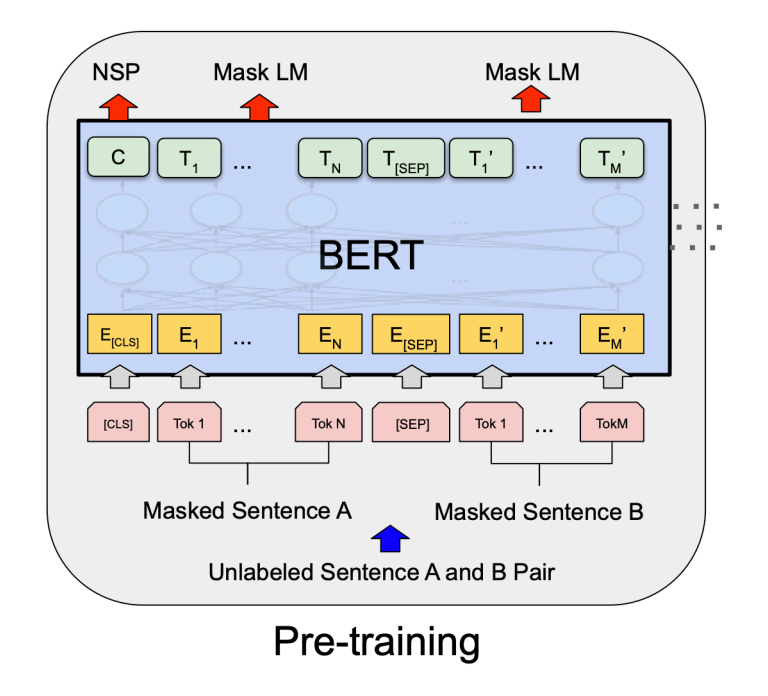
\includegraphics[width=\textwidth]{Figures/BERT-pretraining.png} % Replace with your image path
                \caption*{Pre-training}
            \end{figure}
        \end{column}
    \end{columns}
    \begin{tikzpicture}[remember picture,overlay]
        \node[anchor=south west, xshift=0.09cm, yshift=0.3cm] at (current page.south west) {\tiny \href{https://arxiv.org/abs/1810.04805}{https://arxiv.org/abs/1810.04805}};
    \end{tikzpicture}
\end{frame}

\begin{frame}{Fine-tuning BERT}
    \centering
    \textbf{``Pre-train once, finetune many times.''} \\
    \textcolor{green}{\textbf{token-level tasks}}
    \begin{figure}
        \centering
        % Placeholder for the second image
        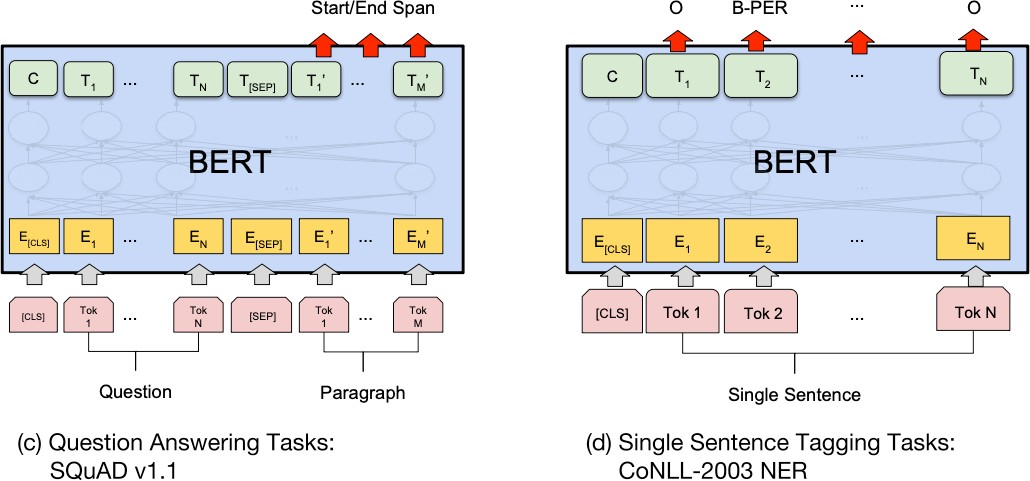
\includegraphics[width=0.7\textwidth]{Figures/Fintuning.png}
    \end{figure}
    For token-level prediction tasks, add linear classifier on top of hidden representations
    \textcolor{green}{Q: How many new parameters?}
\end{frame}

\begin{frame}{Fine-tuning BERT}
    \centering
    \textbf{``Pre-train once, finetune many times.''} \\
    \textcolor{green}{\textbf{sentence-level tasks}}
    \begin{figure}
        \centering
        % Placeholder for the second image
        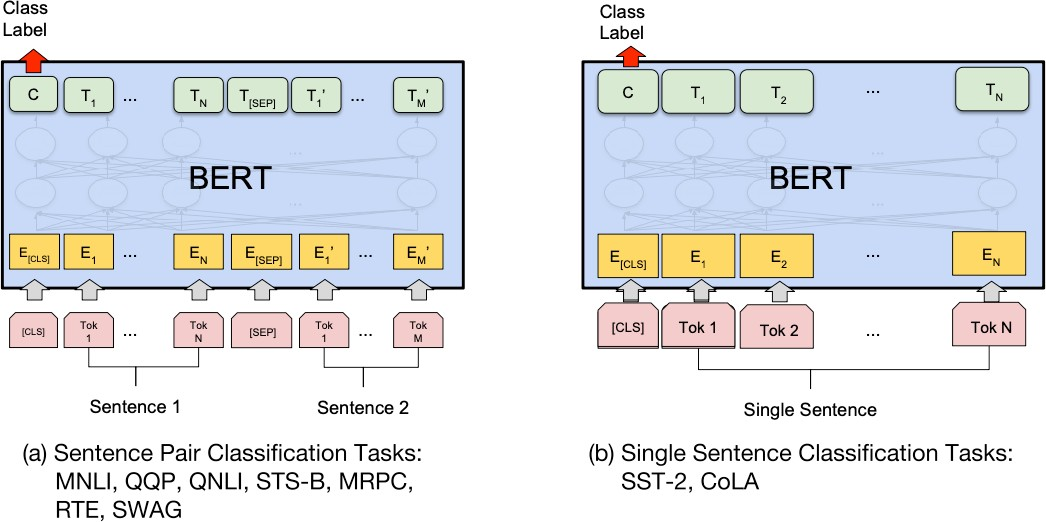
\includegraphics[width=0.7\textwidth]{Figures/finetuning1.png}
    \end{figure}
    For sentence pair tasks, use [SEP] to separate the two segments with segment embeddings and add a linear classifier on top of [CLS] representation.
\end{frame}

\begin{frame}{Finetuning Paradigm in NLP}
    \begin{figure}
        \centering
        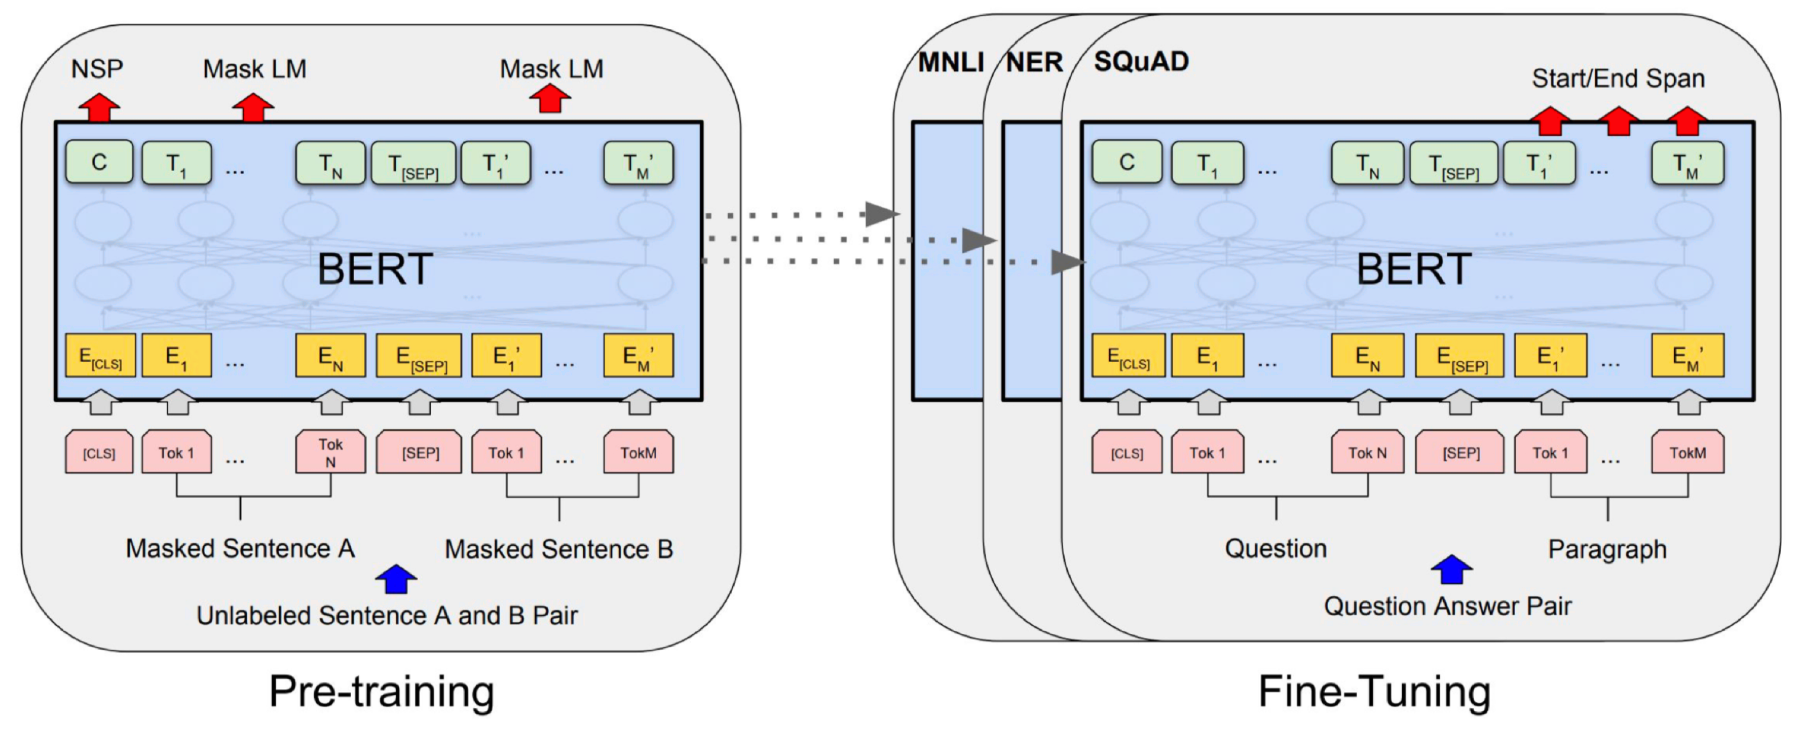
\includegraphics[width=1\textwidth]{Figures/paradaigm.png}
    \end{figure}
\end{frame}

\begin{frame}{BERT Extensions}
    \begin{itemize}
        \item Models that handle long contexts ($> 512$ tokens)
        \begin{itemize}
            \item Longformer, Big Bird, \dots
        \end{itemize}
        
        \item Multilingual BERT
        \begin{itemize}
            \item Trained single model on 104 languages from Wikipedia. Shared 110k WordPiece vocabulary
        \end{itemize}
        
        \item BERT extended to different domains
        \begin{itemize}
            \item SciBERT, BioBERT, FinBERT, ClinicalBERT, \dots
        \end{itemize}
        
        \item Making BERT smaller to use
        \begin{itemize}
            \item DistillBERT, TinyBERT, \dots
        \end{itemize}
    \end{itemize}
\end{frame}

\begin{frame}{BERT Extensions}
    \begin{itemize}
        \item \textbf{RoBERTa} {\color{green}(Liu et al., 2019)}
        \vspace{0.3cm}
        \begin{itemize}
            \item Trained on 10x data \& longer, no NSP
            \item Much stronger performance than BERT (e.g., 94.6 compared to 90.9 on SQuAD)
            \item Still one of the most popular models to date
        \end{itemize}
        \vspace{0.5cm}
        \item \textbf{ALBERT} {\color{green}(Lan et al., 2020)}
        \vspace{0.3}
        \begin{itemize}
            \item Increasing model sizes by sharing model parameters across layers
            \item Less storage, much stronger performance but runs slower
        \end{itemize}
    \end{itemize}
\end{frame}



\section{Decoder Architecture}

\begin{frame}{Decoder Language Model}
    \textbf{Autoregressive (AR)} models use Decoder stacks in generation, aiming to
    maximize log-likelihood via forward autoregressive factorization:
    \begin{figure}
        \centering
        % Placeholder for the second image
        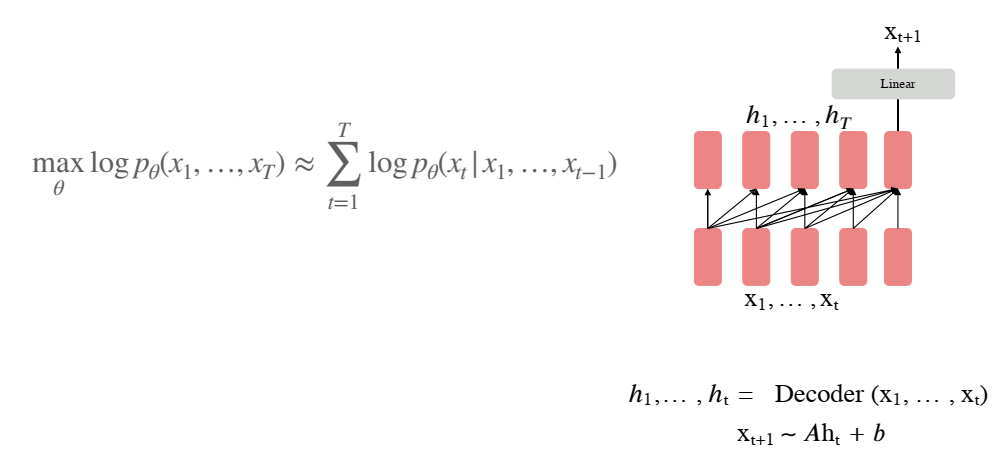
\includegraphics[width=0.9\textwidth]{Figures/decoderlm.png}
    \end{figure}
\end{frame}

\begin{frame}{Decoder Language Model}
    \begin{figure}
        \centering
        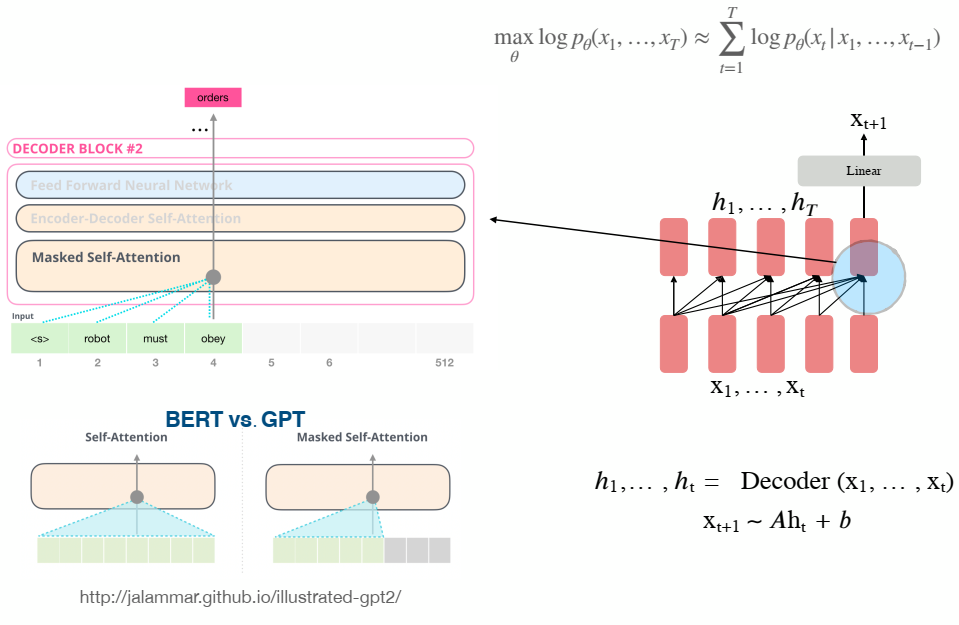
\includegraphics[width=0.8\textwidth]{Figures/decodelm1.png}
    \end{figure}
\end{frame}

\begin{frame}{Generative Pre-Trained Transformer (GPT)}
    \vspace{0.3cm}
    \begin{itemize}
        \item Transformer Decoder with 12 layers.
        \item Byte Pair Encoding (BPE) with 40,000 merges. merges.
        \item Trained on BooksCorpus: over 7000 unique books.
        \begin{itemize}
            \item Contains long spans of contiguous text, for learning long-distance dependencies.
        \end{itemize}
    \end{itemize}
    \begin{figure}
        \centering
        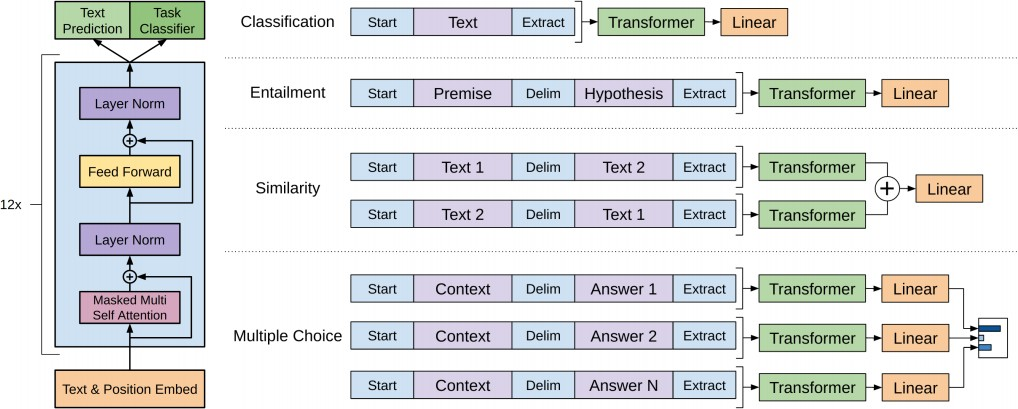
\includegraphics[width=0.8\textwidth]{Figures/GPT.png}
    \end{figure}
    \begin{tikzpicture}[remember picture,overlay]
        \node[anchor=south west, xshift=0.09cm, yshift=0.3cm] at (current page.south west) {\tiny \href{https://www.mdpi.com/2079-9292/13/17/3509}{https://www.mdpi.com/2079-9292/13/17/3509}};
    \end{tikzpicture}
\end{frame}

\begin{frame}{Generative Pre-Trained Transformer (GPT)}
    \begin{figure}
        \centering
        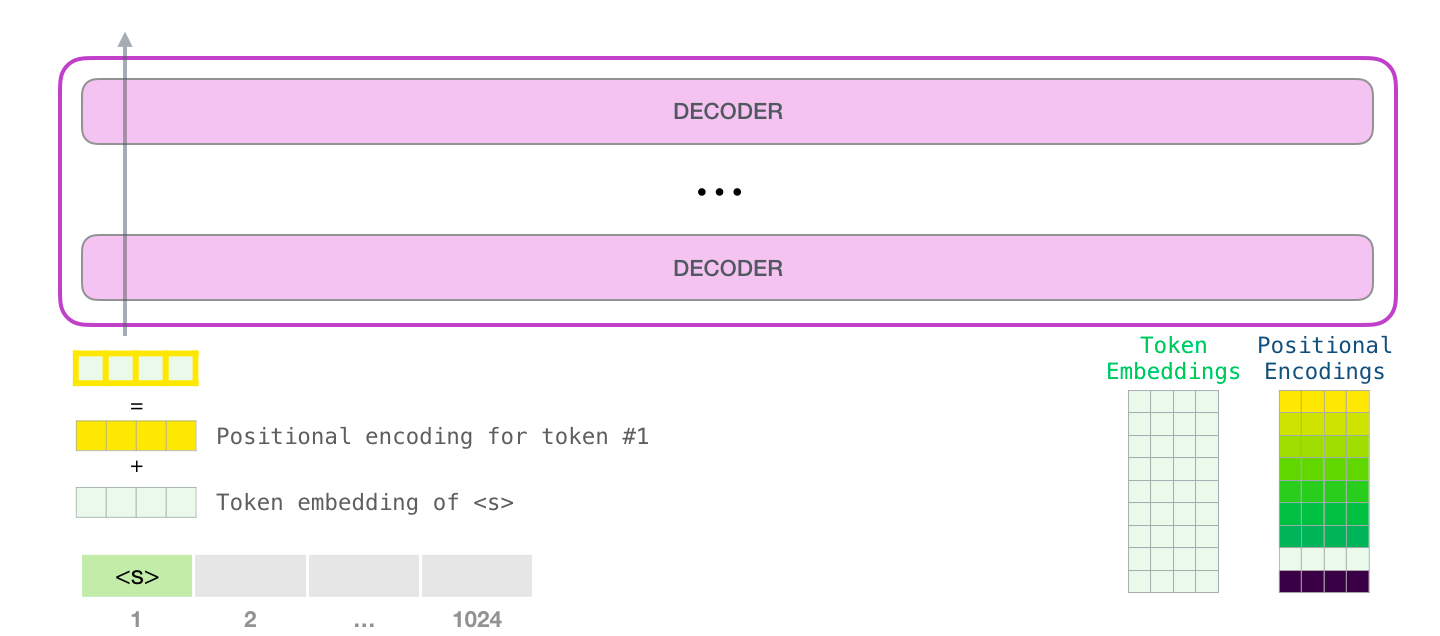
\includegraphics[width=1\textwidth]{Figures/GPT1.png}
    \end{figure}
     \begin{tikzpicture}[remember picture,overlay]
        \node[anchor=south west, xshift=0.3cm, yshift=0.3cm] at (current page.south west) {\tiny \href{https://michaelfu1998-create.github.io/papers/vulrepair.pdf}{https://michaelfu1998-create.github.io/papers/vulrepair.pdf}};
    \end{tikzpicture}
\end{frame}

\begin{frame}{Generative Pre-Trained Transformer (GPT)}
    \begin{figure}
        \centering
        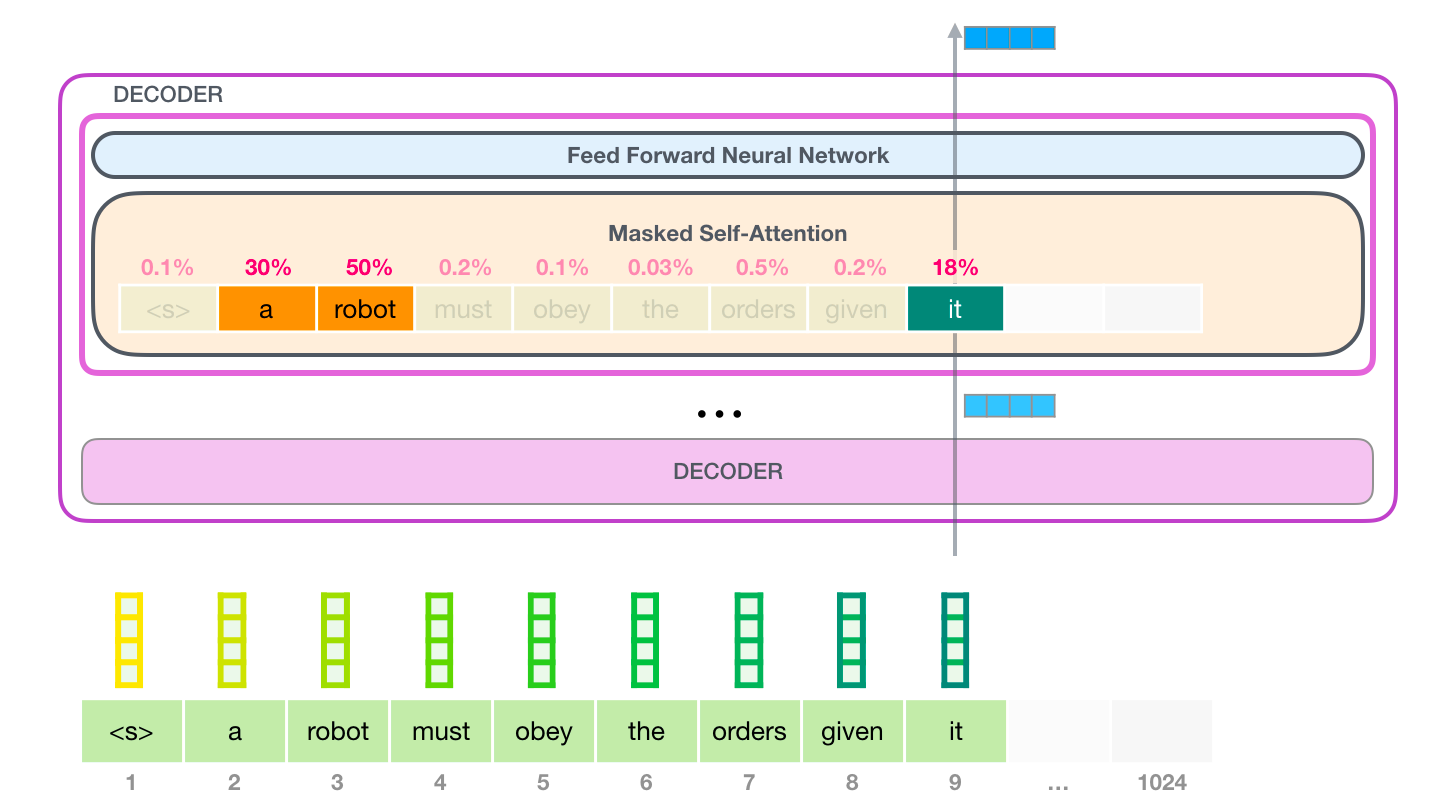
\includegraphics[width=0.8\textwidth]{Figures/GPT2.png}
    \end{figure}
    \begin{tikzpicture}[remember picture,overlay]
        \node[anchor=south west, xshift=0.09cm, yshift=0.3cm] at (current page.south west) {\tiny \href{https://michaelfu1998-create.github.io/papers/vulrepair.pdf}{https://michaelfu1998-create.github.io/papers/vulrepair.pdf}};
    \end{tikzpicture}
\end{frame}

\begin{frame}{Generative Pre-Trained Transformer (GPT)}
    \begin{itemize}
        \item GPT released June 2018
        \item GPT-2 released Nov. 2019 with 1.5B parameters
        \item GPT-3: 175B parameters trained on 45TB texts
    \end{itemize}   
    \begin{figure}
        \centering
        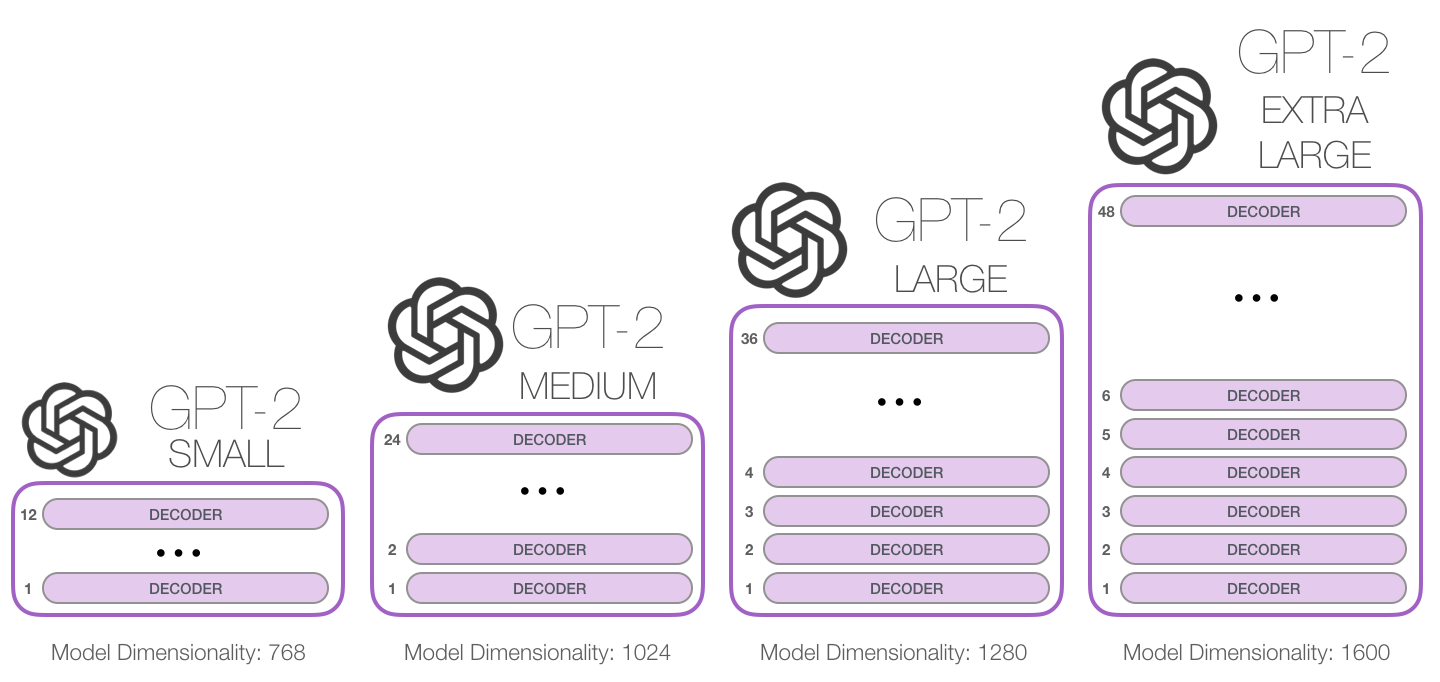
\includegraphics[width=0.8\textwidth]{Figures/GPT3.png}
    \end{figure}
\end{frame}

\begin{frame}{GPT Model Comparison}
    \centering
    \resizebox{\textwidth}{!}{%
        \begin{tabular}{|l|p{5cm}|p{5cm}|}
            \hline
            \textbf{Model} & \textbf{Description} & \textbf{Data} \\
            \hline
            \textbf{GPT-2} (Radford et al., 2019) & Context size: 1024 tokens, 117M-1.5B parameters & WebText (45 million outbound links from Reddit with 3+ karma); 8 million documents (40GB) \\
            \hline
            \textbf{GPT-3} (Brown et al., 2020) & Context size: 2048 tokens, 125M-175B parameters & Common Crawl + WebText + “two internet-based books corpora” + Wikipedia (400B tokens, 570GB) \\
            \hline
        \end{tabular}%
    }
\end{frame}

\begin{frame}{Few-Shot, One-Shot, and Zero-Shot Learning in Language Models}
    \begin{figure}
        \centering
        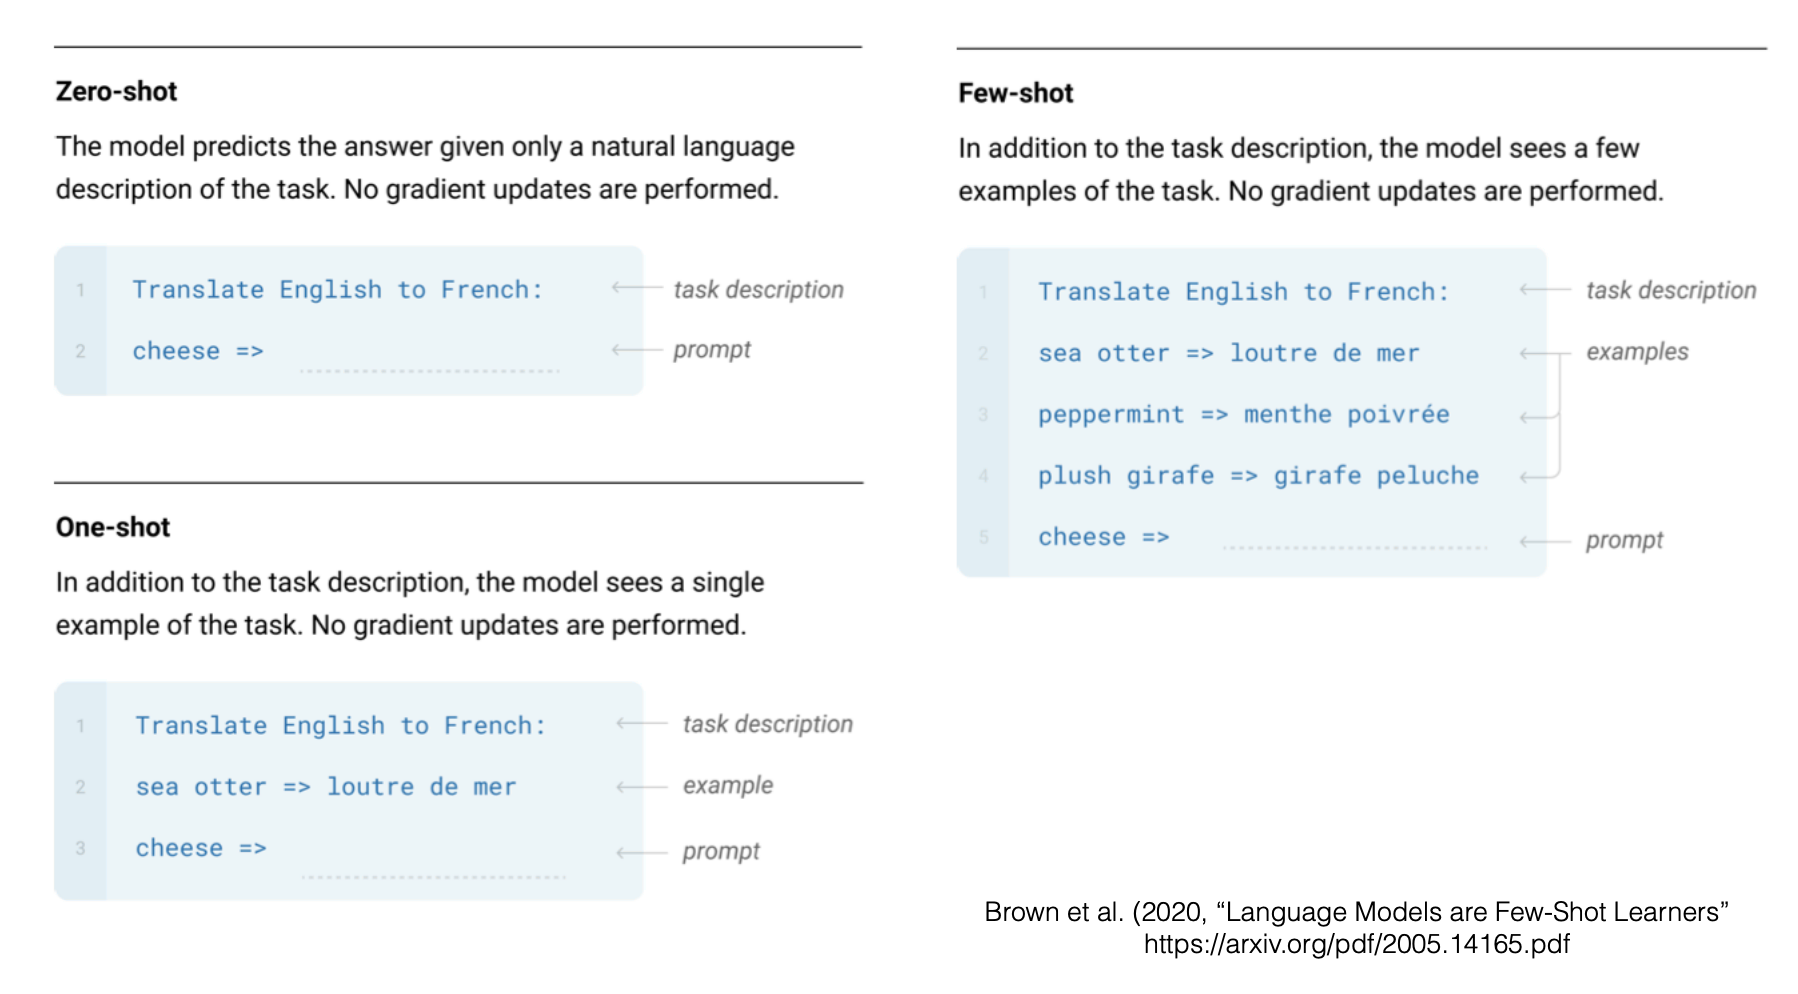
\includegraphics[width=0.9\textwidth]{Figures/fewshot.png}
    \end{figure}
\end{frame}

\section{References}

\begin{frame}[allowframebreaks]{References}
    \footnotesize
    \begin{itemize}
        \item Asgari, E. "Natural language processing." Sharif University of Technology.

        \item Soleymani, M. "Machine learning." Sharif University of Technology.
        \item Radford, A., Wu, J., Child, R., Luan, D., Amodei, D., & Sutskever, I. (2019). "Language Models are Unsupervised Multitask Learners." OpenAI Blog. Retrieved from https://openai.com/research/language-unsupervised

        \item Brown, T. B., Mann, B., Ryder, N., Subbiah, M., Kaplan, J., Dhariwal, P., ... & Amodei, D. (2020). "Language Models are Few-Shot Learners." \textit{arXiv preprint arXiv:2005.14165}.

        \item Liu, Y., Ott, M., Goyal, N., Du, J., Joshi, M., Chen, D., ... & Stoyanov, V. (2019). "RoBERTa: A Robustly Optimized BERT Pre-training Approach." \textit{arXiv preprint arXiv:1907.11692}.

        \item Lan, Z., Chen, M., Goodman, S., Gimpel, K., Sharma, P., & Soricut, R. (2020). "ALBERT: A Lite BERT for Self-supervised Learning of Language Representations." In \textit{Proceedings of the International Conference on Learning Representations (ICLR)}.

        \item Joshi, M., Chen, D., Liu, Y., Weld, D. S., Zettlemoyer, L., & Levy, O. (2020). "SpanBERT: Improving Pre-training by Representing and Predicting Spans." \textit{Transactions of the Association for Computational Linguistics}, vol. 8, pp. 64-77.

        \item Wettig, A., Baykal, C., Ruder, S., & Søgaard, A. (2022). "Should All Tokens be Masked? A Pilot Study of Masked Language Model Performance on Diagnostic Classifiers." \textit{Proceedings of the AAAI Conference on Artificial Intelligence}, vol. 36, no. 10, pp. 10993-11001.

        \item Tjong Kim Sang, E. F., & De Meulder, F. (2003). "Introduction to the CoNLL-2003 Shared Task: Language-Independent Named Entity Recognition." In \textit{Proceedings of the 7th Conference on Natural Language Learning at HLT-NAACL 2003}.

        \item Radford, A., Narasimhan, K., Salimans, T., & Sutskever, I. (2018). "Improving Language Understanding by Generative Pre-Training." Retrieved from https://www.cs.ubc.ca/~amuham01/LING530/papers/radford2018improving.pdf
        
    \end{itemize}
\end{frame}


\end{document}
